\documentclass[11pt,a4paper]{article}

\usepackage[utf8]{inputenc}
\usepackage[T1]{fontenc}
\usepackage[spanish,es-nodecimaldot]{babel}
\usepackage{lmodern}
\usepackage{geometry}
\usepackage{microtype}
\usepackage{xcolor}
\usepackage{booktabs}
\usepackage{tabularx}
\usepackage{array}
\usepackage{enumitem}
\usepackage{fancyhdr}
\usepackage{hyperref}
\usepackage{graphicx}
\usepackage[section]{placeins}
\usepackage{float}

\geometry{left=2.6cm,right=2.6cm,top=2.6cm,bottom=2.6cm}
\definecolor{Azul}{HTML}{17283B}
\definecolor{Rojo}{HTML}{B73739}
\definecolor{Gris}{HTML}{53606B}
\definecolor{Suave}{HTML}{F3F5F7}
\hypersetup{colorlinks=true,linkcolor=Azul,urlcolor=Rojo}
\setlength{\parindent}{0pt}
\setlength{\parskip}{0.55em}
\setlist[itemize]{leftmargin=1.5em,itemsep=0.2em,topsep=0.2em}
\setlist[enumerate]{leftmargin=1.6em,itemsep=0.2em,topsep=0.2em}
\renewcommand{\arraystretch}{1.18}
\newcommand{\codigo}[1]{\texttt{#1}}
\newcommand{\cita}[1]{\textsuperscript{\textcolor{Rojo}{[#1]}}}
\newcommand{\dato}[1]{\textcolor{Azul}{\bfseries #1}}
\graphicspath{{figuras/}}

\pagestyle{fancy}
\fancyhf{}
\fancyhead[L]{\small\textcolor{Gris}{Five Nights of Terror}}
\fancyhead[R]{\small\textcolor{Gris}{Avance final · IHC}}
\fancyfoot[C]{\thepage}
\renewcommand{\headrulewidth}{0.4pt}

\begin{document}

\begin{titlepage}
\thispagestyle{empty}
\addcontentsline{toc}{section}{1. Carátula}
\begin{center}
\vspace*{1.5cm}
{\Large\bfseries Universidad Católica San Pablo\par}
\vspace{0.35cm}
{\large Curso de Interacción Humano--Computador\par}
\vspace{1.8cm}
{\color{Rojo}\rule{0.75\textwidth}{2pt}\par}
\vspace{0.55cm}
{\Huge\bfseries Avance final\par}
\vspace{0.45cm}
{\LARGE Five Nights of Terror\par}
\vspace{0.35cm}
{\large Juego de vigilancia con interacción entre PC, tablet y cámara\par}
\vspace{0.55cm}
{\color{Rojo}\rule{0.75\textwidth}{2pt}\par}
\vspace{1.8cm}
\begin{tabular}{>{\bfseries}p{3.5cm}p{8cm}}
Curso: & Interacción Humano--Computador (CS2H1)\\
Estudiantes: & Marcelo Torres y Anthony Briceño\\
Semestre: & 2026-02\\
Universidad: & Universidad Católica San Pablo\\
\end{tabular}
\vfill
{\large Arequipa, Perú · 2026\par}
\end{center}
\end{titlepage}

\tableofcontents
\clearpage
\setcounter{section}{1}

\section{Descripción del aplicativo}

\textit{Five Nights of Terror} es un prototipo de juego de terror y vigilancia en el que la persona debe sobrevivir desde las 12:00 a.\,m. hasta las 6:00 a.\,m. durante seis noches. La experiencia reparte la atención entre un monitor de PC, donde se ve la escena tridimensional, y una tablet, donde se resuelven minitareas y se controla la caja musical. Una cámara web permite estimar si el jugador dirige la cabeza hacia la pantalla. Si un animatrónico lo alcanza, la noche termina en derrota; al sobrevivir hasta las 6:00 a.\,m. se desbloquea la siguiente, y completar la sexta produce la victoria final.\cita{R1}

El juego propone tres presiones simultáneas. \dato{Freddy} puede avanzar cuando el jugador deja de mirar el PC; \dato{Vixy} se vuelve peligrosa cuando se acumulan tareas sin resolver; y \dato{Puppet} depende del nivel de una caja musical que se vacía con el tiempo. Cada amenaza requiere una respuesta distinta: volver la vista al monitor, completar tareas o dar cuerda a la caja desde la tablet. Esta alternancia es la mecánica central, no un efecto secundario de la interfaz.

El prototipo integra componentes que antes podían ejecutarse de forma separada. En la versión examinada, Unity toma las decisiones sobre tiempo, tareas, movimiento y ataques; Flutter presenta controles y minijuegos; un relay en Python transmite mensajes entre ambos. El informe describe esa versión del proyecto. No presenta resultados de una evaluación formal con participantes, porque no consta una prueba completa de ese tipo en los materiales revisados.
\begin{itemize}
  \item \textbf{Vigilancia con cámara.} MediaPipe Unity Plugin obtiene puntos faciales y el componente \codigo{HeadOrientationTracker} calcula una proporción entre frente, nariz y mentón. El estado booleano \codigo{mirandoPC} se usa para la mecánica de Freddy y para la prueba del tutorial.
  \item \textbf{Escena 3D y enemigos.} Unity 2022.3.30f1 muestra el entorno, mueve los animatrónicos mediante rutas y \codigo{NavMeshAgent}, controla la caja musical, reproduce señales sonoras y presenta los resultados de la partida.
  \item \textbf{Tablet interactiva.} Flutter implementa el menú, el tutorial, la lista de tareas y diez minijuegos: cables, perillas, secuencia, ritmo, WiFi, ventiladores, temperatura, procesamiento de datos, subida de datos y trazado de curso. La caja musical es una acción permanente aparte de esa lista.
  \item \textbf{Comunicación bidireccional.} Unity y Flutter intercambian mensajes JSON mediante WebSocket. \codigo{UnityRelay} los reenvía según el rol de cada conexión; el relay no ejecuta las reglas del juego.
  \item \textbf{Continuidad.} El progreso por noche se almacena en \codigo{PlayerPrefs}. Tras una derrota puede repetirse la noche; tras una victoria se habilita la siguiente hasta la sexta.
\end{itemize}

\begin{center}
\small
\fcolorbox{Azul}{Suave}{\parbox[c][1.5cm][c]{2.6cm}{\centering\textbf{Tablet / Flutter}\\Menú, tareas y controles}}
\quad$\Longleftrightarrow$\quad
\fcolorbox{Azul}{Suave}{\parbox[c][1.5cm][c]{2.1cm}{\centering\textbf{UnityRelay}\\Mensajes JSON}}
\quad$\Longleftrightarrow$\quad
\fcolorbox{Azul}{Suave}{\parbox[c][1.5cm][c]{2.6cm}{\centering\textbf{PC / Unity}\\Reglas, escena y cámara}}
\end{center}

El flujo comienza con \codigo{connect}. Unity inicializa la noche y envía \codigo{task\_list}, \codigo{night\_status} y \codigo{estado\_puppet}. La tablet presenta estos estados y, al terminar una tarea, responde con \codigo{task\_completed} o \codigo{task\_failed}. Unity actualiza el estado de los enemigos y, cuando corresponde, publica \codigo{attack} y \codigo{game\_over}. La cámara se procesa en el PC; el intercambio entre dispositivos se basa en eventos y estados, no en transmitir el video de la webcam.

El uso de WebSocket permite que ambos extremos reciban eventos durante una sesión sin abrir una conexión nueva para cada interacción. El estándar define un canal bidireccional; en el prototipo, el contenido de cada mensaje se expresa como JSON y la lógica de negocio permanece en Unity.

\section{Problemas encontrados y soluciones planteadas}
Durante la última actualización, dejando de lado un poco la parte mecánica, pasamos por las pruebas de los \textit{testers}. Al leer sus comentarios, varios de ellos coincidían en los mismos problemas al usar nuestro juego, como los siguientes:
\begin{itemize}
    \item \textbf{Problema con el script de Windows:} en la creación para la parte de iniciar el juego, creamos scripts para cargar tanto la conexión de la tablet como el inicio de Unity. Este funcionaba perfectamente al crear el \codigo{.ps1}, pero hubo problemas con Windows que no supimos identificar.
    \item \textbf{Respuesta táctil de Puppet:} hubo problemas con el envío de la señal hacia el servidor al presionar el reinicio de la cajita musical (figura~\ref{fig:caja_musical}). El gesto se cancelaba si el dedo se deslizaba unos píxeles y la cuerda se soltaba; ahora la caja musical y la subida de datos leen el toque de forma directa.
    \item \textbf{Tareas sin culminar:} cuando queríamos hacer las tareas de la tablet, estas se salían o regresaban al menú de tareas sin haberlas culminado, y nos aparecían como que no las habíamos hecho, lo que generaba problemas con la interacción del juego. Un claro ejemplo es la tarea de procesar datos: si hacíamos un falso \textit{touch} en un lugar no indicado, se perdía el avance. Ahora un deslizamiento equivocado solo reinicia la secuencia y no termina la tarea.
    \item \textbf{No sabían quién los mató:} uno de los \textit{testers} no lograba identificar qué animatrónico lo había atrapado. La pantalla de derrota ahora dice \textbf{TE ATRAPÓ} seguido del nombre, con su ícono y el motivo (figura~\ref{fig:derrota}): Freddy, por no mirar la pantalla; Vixy, por tener tareas pendientes; y Puppet, por dejar la caja musical sin cuerda.
    \item \textbf{Tablet difícil de leer y de tocar:} la flecha de volver y el botón de cerrar pasaron de 48 a 80 píxeles de lado, se respetó el área segura de la pantalla para que botones como \textit{Enviar} no quedaran tapados, y se agrandaron los textos y los elementos de todos los minijuegos. Además se agregaron avisos por vibración.
    \item \textbf{Cables solo por color:} los cables se distinguían únicamente por su color; ahora cada uno tiene además una forma distinta (figura~\ref{fig:cables}).
    \item \textbf{Las primeras noches eran muy fáciles:} Freddy toleraba entre 35 y 20 segundos sin ser mirado, según la noche, y ahora tolera entre 22 y 12; además, Vixy avanza cada 6 segundos en lugar de cada 8.
    \item \textbf{La tablet decía «Conectado» sin el juego:} el estado cambiaba a conectado al instante, aunque el juego estuviera cerrado. Ahora solo se muestra cuando Unity responde y, si no lo encuentra en 8 segundos, avisa «No se encontró el juego» y permite reintentar. También se corrigieron los textos del tutorial, que estaban escritos en voseo.
\end{itemize}

\begin{figure}[H]
    \centering
    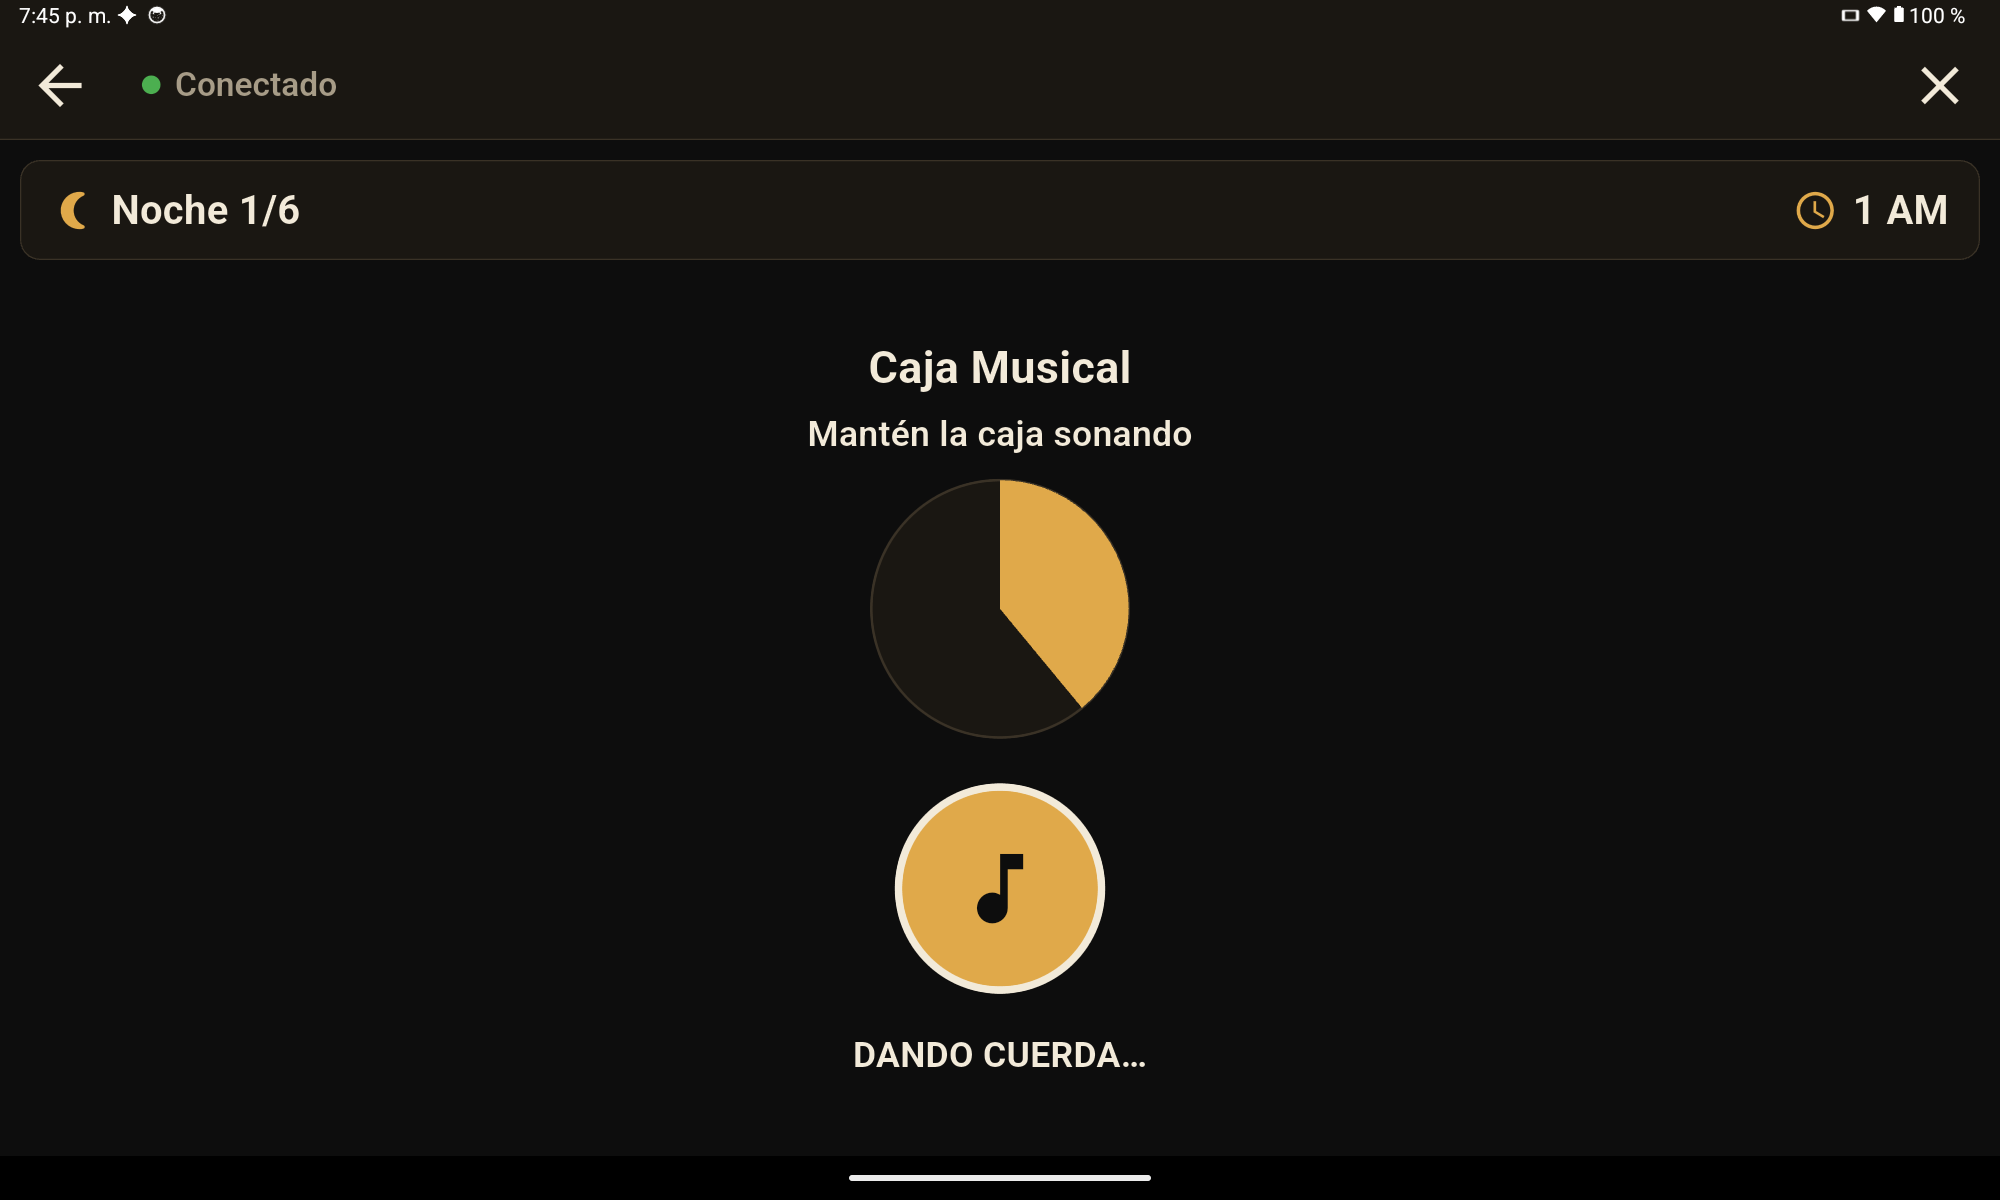
\includegraphics[height=3.6cm]{07_caja_musical.png}\qquad
    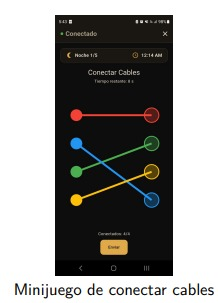
\includegraphics[height=3.6cm]{cables_solo_colores_anterior.png}\quad
    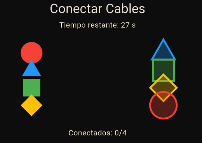
\includegraphics[height=3.6cm]{cables_formas_actual.png}
    \caption{Izquierda: cajita musical con la interfaz cambiada y mejor respuesta táctil. Centro y derecha: cables solo por color y con formas}
    \label{fig:caja_musical}\label{fig:cables}
\end{figure}

\section{Discusión sobre las opiniones de los individuos de prueba}
Este apartado se centrará en la discusión sobre las opiniones de mejora de nuestro juego que dieron los \textit{testers}.

Algo en que coincidían muchos de los \textit{testers} era que a veces, cuando interactuaban con la tablet para hacer las minitareas, estas no respondían. Podía ser un problema de que no presionaban en los lugares clave o simplemente que el servidor no recibía la señal del \textit{touch}.

También hicieron énfasis en la parte del screamer del animatrónico, ya que sentían que era lo esencial en este estilo de juegos. Dicho esto, agregamos un video como parte final al recibir un screamer, como en la figura~\ref{fig:fredy}.

Los videos de Freddy y de Puppet fueron generados con una herramienta de inteligencia artificial generativa (Gemini)\cita{R6}, a partir de imágenes de los propios modelos del juego, y luego recortados al fragmento del salto. El de Vixy no usó inteligencia artificial: se elaboró con un programa propio que anima su imagen con acercamiento, temblor y destellos. En los tres casos el sonido es el del juego.

Algunos se enfocaron en las mecánicas y en cómo aprovecharlas. Por ejemplo, si la tablet se ponía a una altura en que la cámara pudiera detectar la frente o el mentón, figuraba como \textit{true}; de este modo, Freddy, que depende de la cámara para atacar, no realizaba movimientos. Por eso planteamos que el videojuego se base en tener la tablet a un costado, para evitar este tipo de pérdidas de experiencia.

\clearpage
\begin{figure}[H]
    \centering
    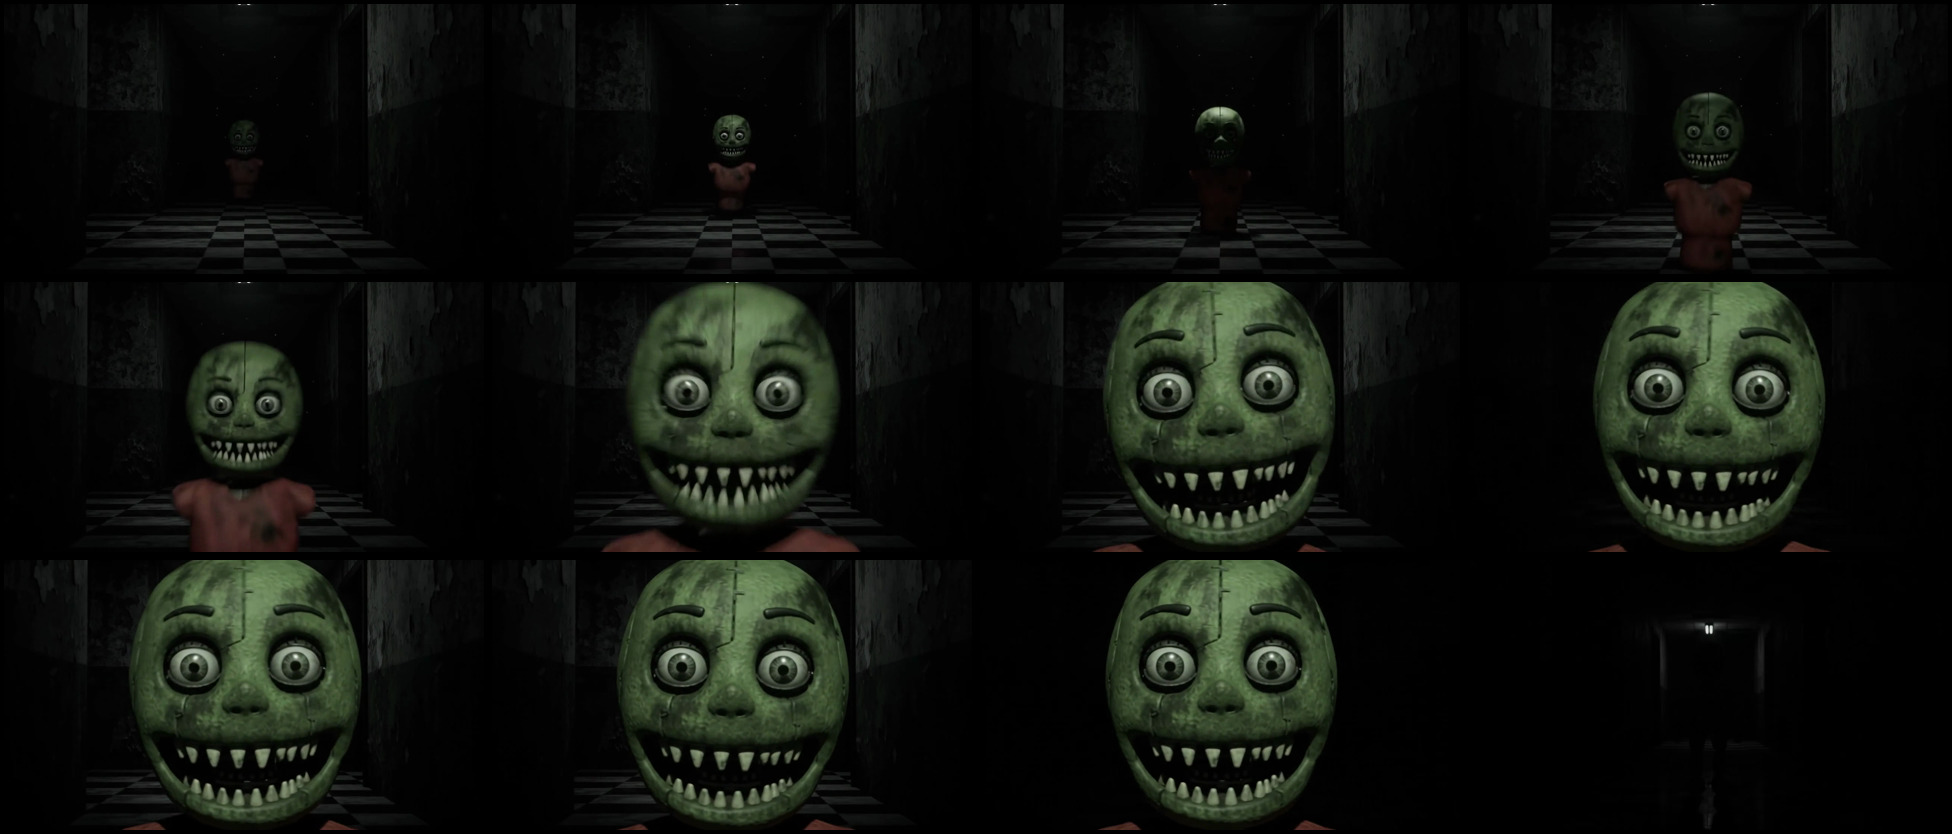
\includegraphics[height=3.4cm]{jumpscare_freddy_secuencia.jpg}\qquad
    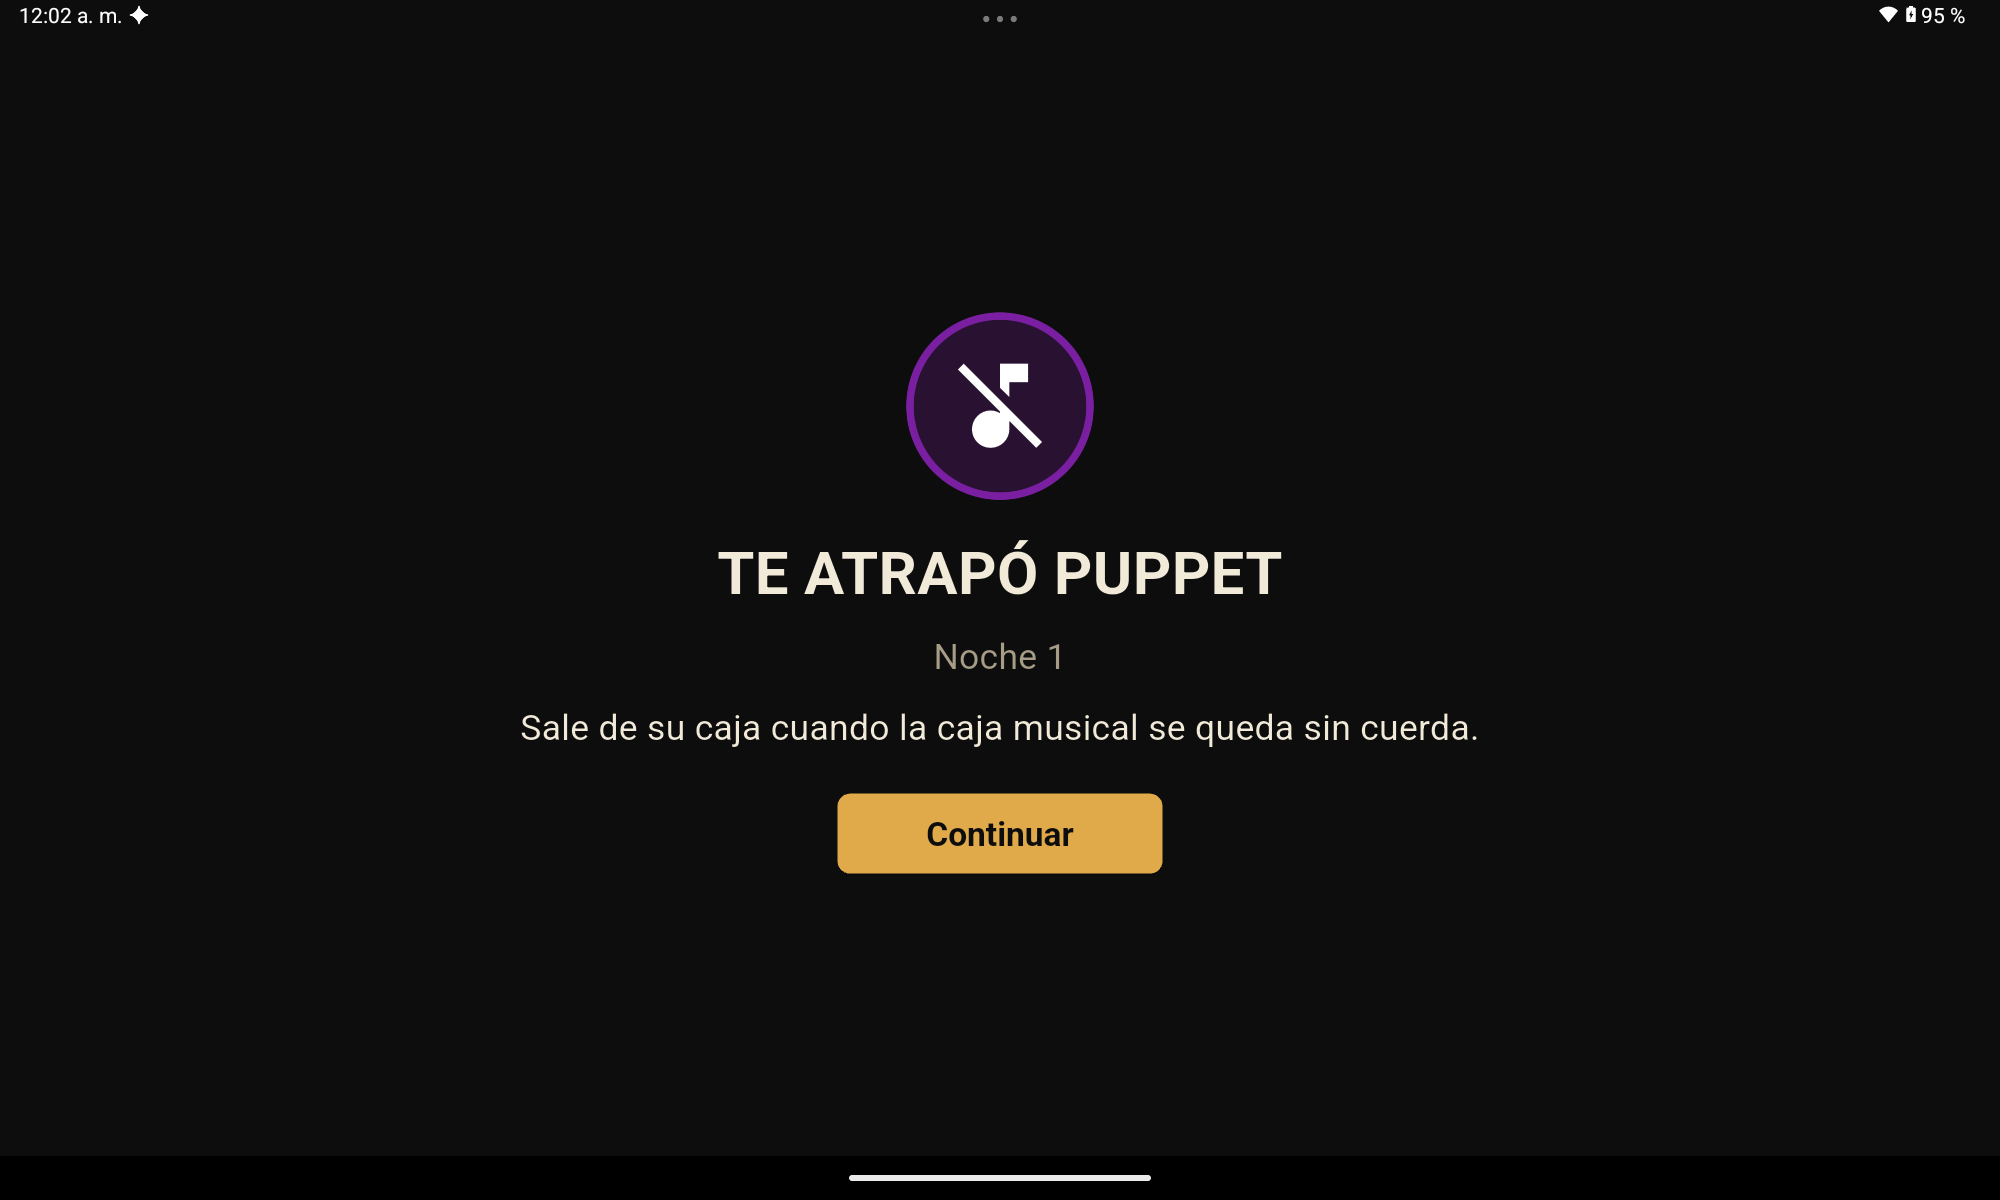
\includegraphics[height=3.4cm]{12_te_atrapo_puppet.png}
    \caption{Izquierda: jumpscare de Freddy. Derecha: pantalla de derrota en la tablet, que indica qué animatrónico atrapó al jugador}
    \label{fig:fredy}\label{fig:derrota}
\end{figure}

\section{Conclusiones}

\begin{enumerate}
  \item El prototipo logra integrar vigilancia en PC, minitareas en tablet y detección de rostro en una misma dinámica. Unity concentra las reglas y el relay mantiene el intercambio entre dispositivos, lo que permite describir con claridad el origen de cada evento.
  \item El tutorial de tres pantallas transforma las instrucciones en una pequeña práctica: muestra la cámara real y permite probar una tarea antes de comenzar. Es una mejora de comprensión y preparación, aunque su eficacia debe comprobarse con jugadores nuevos.
  \item La especificidad del sistema genera sus principales límites. La cámara no equivale siempre a intención de mirar; la alternancia de pantallas añade carga cognitiva, y algunos gestos temporizados o sostenidos no ofrecen todavía una alternativa. La corrección de cables mediante formas demuestra que una limitación puede mitigarse con cambios concretos de interfaz.
  \item Las correcciones hechas a partir de los comentarios de los \textit{testers} (respuesta táctil, identificación del animatrónico que ataca, dificultad y jumpscare) atienden los problemas observados, pero todavía deben validarse con nuevos jugadores para confirmar que resuelven la experiencia.
  \item Como trabajo posterior se recomienda evaluar partidas completas con participantes, registrar pérdidas de detección y tiempos de tarea, probar distintas cámaras y condiciones de luz, y revisar señales redundantes y opciones de accesibilidad. Estas son recomendaciones de validación, no resultados ya medidos.
\end{enumerate}

\clearpage
\section{Referencias bibliográficas}

\begin{description}[leftmargin=0pt,labelwidth=1.1cm,style=nextline,itemsep=0.75em]
 
  \item[{[R1]}] Flutter. (2026). \textit{Building user interfaces with Flutter}. \url{https://docs.flutter.dev/ui}. 
  \item[{[R2]}] MediaPipe Unity Plugin. (s.\,f.). \textit{Repositorio del proyecto}. \url{https://github.com/homuler/MediaPipeUnityPlugin}. 
  \item[{[R3]}] Unity Technologies. (2022). \textit{NavMesh Agent, Unity Manual 2022.3}. \url{https://docs.unity3d.com/2022.3/Documentation/Manual/class-NavMeshAgent.html}. 
  \item[{[R4]}] Fette, I. y Melnikov, A. (2011). \textit{The WebSocket Protocol}. RFC 6455. Internet Engineering Task Force. \url{https://www.rfc-editor.org/info/rfc6455/}.
  \item[{[R5]}] World Wide Web Consortium. (s.\,f.). \textit{Understanding Success Criterion 1.4.1: Use of Color}. Web Content Accessibility Guidelines 2.2. \url{https://www.w3.org/WAI/WCAG22/Understanding/use-of-color.html}. 
  \item[{[R6]}] Google. (2026). \textit{Gemini}. \url{https://gemini.google.com}.
\end{description}

\end{document}
